
% =============================================================================
% =============================================================================
% =============================================================================
\section{Spatial Distribution of Energy}
  \label{sec_shells}

Looking a bit deeper, it's possible to comment on the structure of the poloidal and toroidal modes, not just their magnitudes. The following commentary addresses the dayside; on the nightside, there's never much by the way of resonance. 

In \cref{fig_resonant_driving,fig_nonresonant_driving}, electromagnetic energy is binned by field line, averaged over volume (again, with respect to the Jacobian), and plotted as contours. All plots share a color scale. 

The poloidal mode and the toroidal mode exhibit qualitatively different behavior, related to the fact that energy rotates from poloidal to toroidal, and not back. 

At low \azm, energy rotates out of the poloidal mode so quickly that no resonance can form. 

At high \azm, the \Alfven wave is guided. If the driving frequency lines up with the resonant frequency where it's delivered, the poloidal mode resonates strongly. Otherwise, again, no energy accumulates. 

In no case does the poloidal mode demonstrate the ability to move energy across magnetic field lines. 

On the other hand, the toroidal mode does resonate, even if the driving isn't resonant (though in that case the response is of course stronger). The toroidal mode transports energy across field lines until it encounters resonance, then accumulates energy there. Often, resonances are seen in multiple locations due to the non-monotonic \Alfven bounce frequency (recall \cref{fig_fa}) as a function of $L$. 

% -----------------------------------------------------------------------------
% -----------------------------------------------------------------------------
% -----------------------------------------------------------------------------
\subsection{Resonant Driving}

\begin{figure}[H]
    \centering
    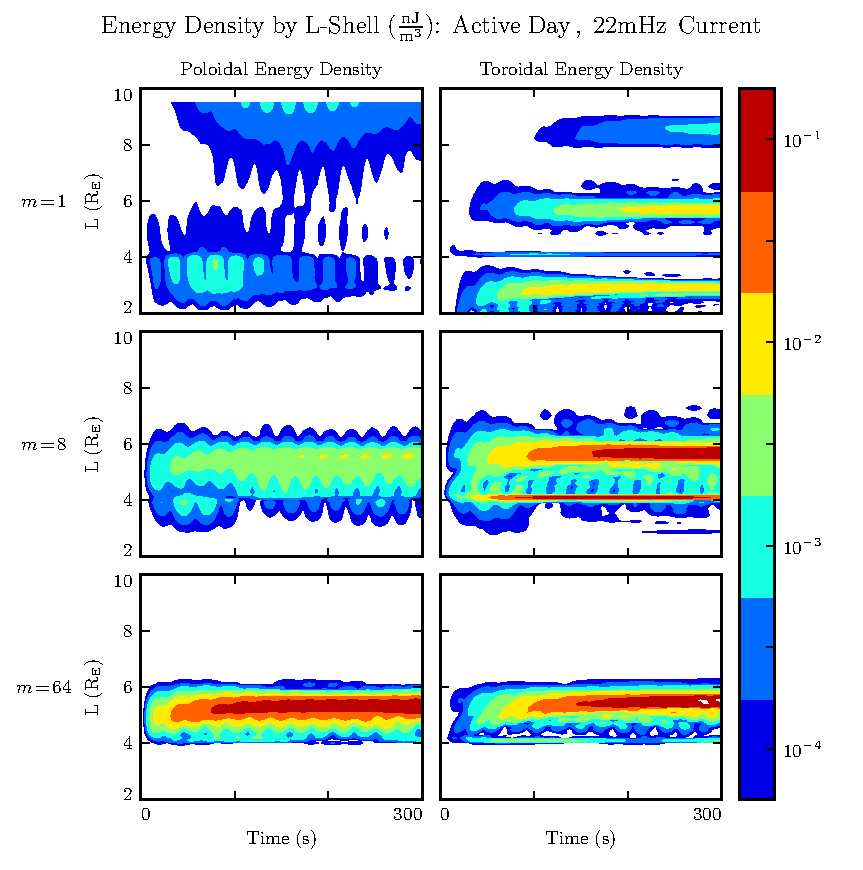
\includegraphics[width=\textwidth]{figures/layers_22mHz_1.pdf}
    \caption[Poloidal and Toroidal Energy Distribution: Resonant Driving]{
      If \azm is small, energy rotates to the toroidal mode too fast to form a poloidal resonance. If \azm is large, the \Alfven wave is guided, so it resonates only if the driving frequency lines up with the resonant frequency where it's applied. The result is just one big -- or perhaps even giant -- pulsation. If the driving lines up with a nearby field line, the toroidal mode goes crazy! Resonance inside the plasmasphere. Resonance at the plasmapause. Resonance at the driving location. And (weak) attempt at a higher harmonic further out. 
    }
    \label{fig_resonant_driving}
\end{figure}

\todo{Why is this exciting? }

\todo{Driving from inside the magnetosphere is novel. }

% -----------------------------------------------------------------------------
% -----------------------------------------------------------------------------
% -----------------------------------------------------------------------------
\subsection{Nonresonant Driving}

\begin{figure}[H]
    \centering
    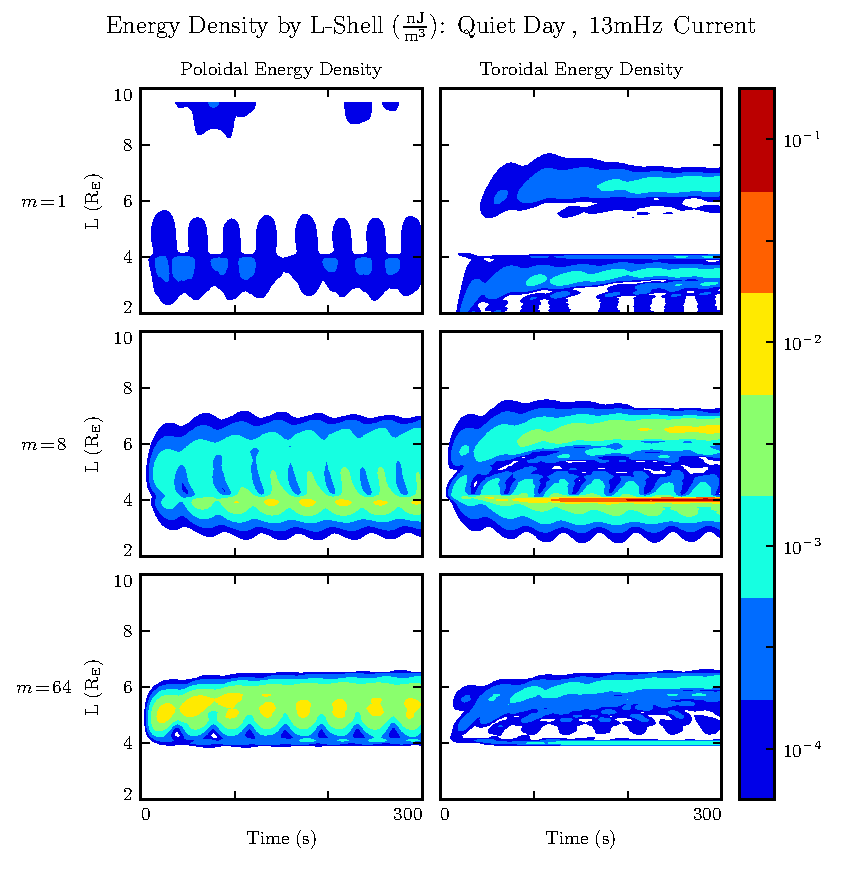
\includegraphics[width=\textwidth]{figures/layers_13mHz_2.pdf}
    \caption[Poloidal and Toroidal Energy Distribution: Nonresonant Driving]{
      When the driving frequency doesn't line up with the location where it's delivered, there's basically no response. There is no movement of energy to a resonant field line, so no energy can accumulate over the course of multiple rounds of driving. Even when not driven resonantly, the toroidal mode still makes the best of its situation. It steals what energy it can from the poloidal mode, carries it to the resonant $L$-shell, and gets to work. (In contrast, recall from \cref{fig_resonant_driving}, in this situation the poloidal mode just does not accumulate energy.)
    }
    \label{fig_nonresonant_driving}
\end{figure}

\todo{Why is this exciting? }

